\documentclass{article}

\linespread{1.1}
\usepackage[utf8]{inputenc} 
\usepackage[T1]{fontenc}
\usepackage[francais]{babel}
\usepackage{amsmath}
\usepackage{amsfonts}
\usepackage{amssymb}
\usepackage{graphicx}
\usepackage{lmodern}
\usepackage{microtype}
\usepackage{hyperref}
\usepackage[margin=1.8cm]{geometry}
\usepackage{pgf,tikz}
\usepackage{mathrsfs}
\usetikzlibrary{arrows}


% Structure

\newcounter{c}
\newcounter{d}
\newcounter{r}
\newcounter{e}

\newcommand{\defi}{\subparagraph{Definition \arabic{c}.\arabic{d} :}\stepcounter{d}}
\newcommand{\prop}{\subparagraph{Proposition \arabic{c}.\arabic{r} :}\stepcounter{r}}
\newcommand{\thm}{\subparagraph{Theorem \arabic{c}.\arabic{r} :}\stepcounter{r}}
\newcommand{\demo}{\subparagraph{Proof}}
\newcommand{\cor}{\subparagraph{Corollary \arabic{c}.\arabic{r} :}\stepcounter{r}}
\newcommand{\lem}{\subparagraph{Lemma \arabic{c}.\arabic{r} :}\stepcounter{r}}
\newcommand{\rem}{\subparagraph{Remark :}}
\newcommand{\chapitre}[1]{\stepcounter{c}\setcounter{e}{0}\setcounter{d}{0}\setcounter{r}{0}\noindent\textbf{\Large#1}\\}
\newcommand{\eq}[1]{\stepcounter{e}\begin{equation}#1\tag{\arabic{c}.\arabic{e}}\end{equation}}

% Notations

\newcommand{\Q}{\mathbb{Q}}
\newcommand{\Z}{\mathbb{Z}}
\newcommand{\N}{\mathbb{N}}
\newcommand{\R}{\mathbb{R}}
\newcommand{\C}{\mathbb{C}}
\newcommand{\E}[1]{\mathbb E\left(#1\right)}
\newcommand{\sph}{\mathbb{S}}
\newcommand{\p}{{\cal{P}}}
\newcommand{\fsp}{{\cal{F}}}
\newcommand*{\qed}{\hfill\ensuremath{\square}}
\newcommand{\x}{\mathbf x}
\newcommand{\y}{\mathbf y}
\newcommand{\e}{\mathbf e}
\newcommand{\scal}[2]{\langle#1,#2\rangle}
\newcommand{\trans}{^\text{T}\!}
\newcommand{\dt}{\frac d{dt}}

\newcommand{\dpart}[2]{\displaystyle\frac{\partial#1}{\partial #2}}

\newcommand{\nor}[2]{{\cal N}(#1,#2)}
\newcommand{\mat}[2]{{\cal M}_{#1\times#2}(\R)}

\newcommand{\X}{\mathbf X}

\renewcommand{\leq}{\leqslant}
\renewcommand{\geq}{\geqslant}

\newcommand{\vertiii}[1]{{\left\vert\kern-0.25ex\left\vert\kern-0.25ex\left\vert #1\right\vert\kern-0.25ex\right\vert\kern-0.25ex\right\vert}}


\newcommand{\mo}{\text{model}}
\newcommand{\spa}{\text{span}}

\begin{document}

\begin{center}\Large\bf
Méthodes des bases réduites pour la qualité de l'air en milieu urbain


\large-
 

J.K. Hammond\end{center}

\bigskip


\chapitre{Parameter Background Data Weak}
\paragraph{Motivation}~


In order to evaluate a quantity of interest $f(u)$ where $f$ is a linear functional, we want to :
\begin{itemize}
\item approximate $u^{true}(\mu)$  for varying parameter $\mu\in\mathcal D$
\item correct approximation using measurements
\end{itemize}



\begin{center}\begin{tabular}{ccccc}approximation& $=$ &model state& + &update term\\

$u^{true}(\mu)$& $\simeq$ &$u^\mo(\mu)$& + &$\eta(\mu)$
\end{tabular}\end{center}


where $u^{true}(\mu)$ is the solution of our PDE's FE formulation supposedly in the form : $$a(u,v;\mu)=f(v;\mu)$$



We have $M$ measurements linearly depending on the true state : $$y^{obs}_m(\mu)=l_m(u^{true}(\mu))$$
 

\paragraph{Parameter Background Data Weak}~



\textbf{Offline RBM :}
\begin{enumerate}
\item choose $N$ snapshots $u(\mu_i),i=1,...,N$ (e.g. with Greedy Algorithm)
\item apply Gram-Schmidt to orthonormalize them : $(\zeta_i)_{i=1,...,N}$
\item define background space $\mathcal X_N=\spa\{\zeta_i,i=1,...,N\}$ with orthonormal basis
%\item project the problem onto $X_N$ : 
%$$X\ni u\mapsto\mathbf u_N(\mu)=(\mathbf u_N^i(\mu))_{i=1,...,N}=((u(\mu),\xi_i)_X)_{i=1,...,N}\in X_N$$
%$$A_N(\mu) = (a(\xi_i,\xi_j;\mu))_{i,j=1,...,N}\text{ and }L_N(\mu) = (l(\xi_i;\mu))_{i=1,...,N}$$
%\item variable separation through affine approximation : $$a(\cdot,\cdot;\mu)\simeq\sum_{q=1}^{Q_a}\theta^a_q(\mu)a_q(\cdot,\cdot)\text{ and }f(\cdot;\mu)\simeq\sum_{q=1}^{Q_f}\theta^f_q(\mu)f_q(\cdot)$$
%\item computation of matrices $\mathbf A_q=(a_q(\xi_i,\xi_j))_{i,j=1,...,N}$, $q=1,...,Q_a$ and $\mathbf F_q=(f_q(\xi_i))_{i=1,...,N}$, $q=1,...,Q_f$
\end{enumerate}



\textbf{Offline update space computations :}
\begin{enumerate}
\item find Riesz' representent of $l_m:X\to X$, $m=1,...,M$ : $$q_m\in X\text{ s.t. }(v,q_m)_X=l_m(v), \forall v\in X$$
\item build update space : $$\mathcal U_M=\spa\{q_m|m=1,...,M\}$$
\item compute matrices : $$\mathbf A=((q_i,q_j)_X)_{i,j=1,...,M}\text{ and }\mathbf B=((\zeta_i,q_j)_X)_{i=1,...,N ; j=1,...,M}$$
\end{enumerate}
 


\textbf{Offline output computations :}


Build the vector $\mathbf f \in\R^{M+N}$ where $\mathbf f_m = f(q_m),~m=1,...,M$ and $\mathbf f_{M+n} = f(\zeta_n),~n=1,...,N$.


\textbf{Online computations :}


Finding the smallest correction $\eta\in\mathcal U_M$ s.t. $y^{obs}_m=(u^{true},q_m)_X=(u_{N,M},q_m)_X$ amounts to require the correction $\eta$ to be in $\mathcal U_M\cap\mathcal X_N^\perp$. We just have to solve a linear system for each set of observations : $$\left(\begin{matrix}\mathbf A&\mathbf B\\\mathbf B^T&\mathbf 0\end{matrix}\right)\left(\begin{matrix}\mathbf n_M\\\mathbf z_N\end{matrix}\right)=\left(\begin{matrix}\mathbf y^{obs}\\\mathbf 0\end{matrix}\right)$$

or for more stability : $$\mathbf B^T\mathbf A^{-1}\mathbf B\mathbf z_N=\mathbf B^T\mathbf A^{-1}\mathbf y^{obs}\text{ and }\mathbf n_M=\mathbf A^{-1}(\mathbf y^{obs}-\mathbf B\mathbf z_N)$$


where $z_N=\mathbf z_N^T\cdot (\zeta_n)_{n=1,...,N}\in\mathcal X_N$ is the RB approximation of $u^{true}$ and $\eta_M=\mathbf n_M^T\cdot(q_m)_{m=1,...,M}\in\mathcal U_M$ is the observation correction. Our best approximation is  $u_{N,M}=z_N+\eta_M$. It only remains the output's evaluation :

$$f(u(\mu))\simeq\mathbf f^T\cdot\left(\begin{matrix}\mathbf n_M\\\mathbf z_N\end{matrix}\right)$$



\textbf{Computational cost :}

The linear system costs $\mathcal O((M+N)^3)$ to solve, and the factorized formulation only costs $\mathcal O((M+N)^2)$ to solve. However, it may be interesting to compute an orthonormalized basis $(\upsilon_m)_{m=1,...,M}$ for $\mathcal U_M$ so $\mathbf A$ would be a diagonal matrix.





\paragraph{Stability and error estimation}~


According to the author, the stability of the PBDW method strongly depends on the inf-sup constant $\beta_{N,M}$ :

$$\beta_{N,M} = \inf_{w\in\mathcal X_N}\sup_{v\in\mathcal U_M}\frac{(w,v)_\mathcal X}{\|w\|_\mathcal X\|v\|_\mathcal X}$$

The \emph{a priori} error bound can be written :

$$\|u^{true}-u_{N,M}\|_\mathcal X\leq\left(1+\frac1\beta_{N,M}\right)\inf_{q\in\mathcal U_M}\inf_{z\in\mathcal X_N}\|u^{true}-z-q\|_{\mathcal X}$$

It would be insteresting to maximize $\beta_{N,M}$ with respect to $M$ and to minimize the correction error $\|P_{\mathcal X_N^\perp}(u^{true})-\eta\|_\mathcal X$ where $P_\mathcal{X_N^\perp}:\mathcal X\to\mathcal X_N^\perp$ is the projection onto $\mathcal X_N^\perp$. The may be done using a greedy-type algorithm among a fine set of possible locations for the $M$ sensors.











%
%
%
%
%
%
%
%\section{Réduction de modèle}
%\paragraph
%\begin{center}\textbf{\Large Réduction de modèle}\end{center}
%\vfill
%Ranine Tarabay : \emph{Modeling of blood flow in complex vascular networks.} Mathematics. Université de Strasbourg, 2016.
%
%\vspace{0.5em}
%
%Christophe Prud'homme : cours CSMI 2016
%
%\vspace{0.5em}
%
%Janelle K. Hammond : \emph{Méthodes des bases réduites pour la qualité de l’air en milieu urbain.} Mathématiques appliquées. IFSTTAR, 2017.
% 
%
%\paragraph
%\frametitle{Problème}
%
%\begin{itemize}
%\item$\Omega\subset\R^d$ un domaine fermé 
%\item$\mathcal D\subset\R^P$ un ensemble de paramètres $\mu$
%\item$\mathcal H^1_0(\Omega)\subset X\subset\mathcal H^1(\Omega)$ un espace de Hilbert complet muni de $\langle\cdot,\cdot\rangle_X$
%\item$l:X\times\mathcal D$ une forme linéaire paramétrique
%\item$a:X\times X\times\mathcal D$ une forme bilinéaire paramétrique
%\item$\mu$ fixé, évaluer la sortie du système (mesure) : $s(\mu)=f(u(\mu);\mu)$ où $u(\mu)\in X$ satisfait : $$a(u(\mu),v;\mu)=l(v;\mu)~~\forall v\in X.$$
%
%
%\end{itemize}
% 
%
%
%
%
%
%
%
%\paragraph{Méthode de la base réduite (RBM)}
%
%\begin{block}<2-3>\defi Soit la variété des solutions du problème FEM :
%$$\mathcal S_\mathcal N=\left\{u_\mathcal N(\mu)~|~\mu\in\mathcal D\right\} \subset X_\mathcal N\subset X$$\end{block}
%
%On approxime $X_\mathcal N$ par un espace "plus simple".
%
%
%Soit $N\in\N$. Soit $\left\{\mu_i~|~i=1,...,N\right\}$.
%
%\begin{block}<3>\defi $$S_N=\left\{u(\mu_i)\in X_\mathcal N~|~i=1,...,N\right\}\subset\mathcal S_\mathcal N$$
%$$X_N=\text{span}(S_N)$$\end{block}
% 
%
%\paragraph{Méthode de la base réduite (RBM)}
%
%\centering\begin{tabular}{p{3cm}}\centering Gram-Schmidt\\sur $S_N$\end{tabular}$\longrightarrow$ \begin{tabular}{p{5cm}}\centering$(\zeta_i~|~i=1,...,N)$\\base orthonormée de $X_N$\end{tabular}
%
%
%\begin{block}{\textbf{Proposition :}}$\forall w\in X_N$, $\exists w_i,i=1,...,N$ : ~~~~~~$w=\displaystyle\sum_{i=1}^Nw_i\zeta_i=\mathbf w^\text T\cdot Z_N$ \end{block}
%
%\begin{block}\defi $$A_N(\mu) = (a(\zeta_i,\zeta_j;\mu))_{i,j=1,...,N}\text{ et }L_N(\mu) = (l(\zeta_i;\mu))_{i=1,...,N}$$\end{block}
%
% 
%
%\paragraph{Méthode de la base réduite (RBM)}
%\begin{block}{\textbf{Réduction :}}
%$$\begin{array}{rcl}
%X&\rightarrow&X_N\\
%u\in X&\rightarrow&\mathbf u_N\in\R^N\text{ t.q. }\mathbf u_N\cdot Z_N^\text T=u_N\\
%a(u,v;\mu)=l(v;\mu)&\rightarrow&\mathbf u_N^\text T\cdot A_N(\mu)\cdot\mathbf v_N = L_N(\mu)^\text T\cdot\mathbf v_N\\
%\end{array}$$
%\end{block}
%
%\bigskip
%
%Comme l'égalité vaut $\forall \mathbf v_N\in X_N$, on se ramène à la résolution du système linéaire :
%$$A_N(\mu)^\text T\cdot\mathbf u_N=L_N(\mu)$$
% 
%
%
%
%\paragraph{Greedy algorithm}
%
%\begin{block}\defi $$\begin{array}{lrccc}\Delta_N&:&\mathcal C&\longrightarrow&\R_+\\&&\mu&\longmapsto&\left\|u(\mu)-\mathbf u_N(\mu)\cdot Z_N^\text T\right\|_X\end{array}$$\end{block}
%
%$Z_N=\{\zeta_i~|~i=1,...,N\}$ étant construite
%\begin{itemize}
%\item<1-3>$\mu_{N+1}=\displaystyle\argmax_{\mu\in\mathcal D}\left(\Delta_N(\mu)\right)$
%\item<2-3>Gram-Schmidt sur $Z_N\wedge u(\mu_{N+1})\longrightarrow\zeta_{N+1}$
%\item<3>$Z_{N+1}=Z_N\wedge\zeta_{N+1}$
%\end{itemize}
% 
%
%\paragraph{Optimalité}
%\begin{block}\defi $a(\cdot,\cdot;\mu)$ est coercive si : $$\alpha(\mu)=\inf_{v\in X}\frac{a(v,v;\mu)}{\left\|v\right\|_X^2}>0$$ et continue si : $$\gamma(\mu)=\sup_{v\in X}\sup_{w\in X}\frac{a(v,w;\mu)}{\left\|v\right\|_X\left\|w\right\|_X}<\infty$$\end{block}
%\begin{block}{\textbf{Proposition :} Galerkin} Si $a(\cdot,\cdot;\mu)$ est une forme bilinéaire, continue, coercive $\forall \mu\in\mathcal D$ : $$\left\|u(\mu)-u_N(\mu)\right\|_X\leqslant\sqrt{\frac{\gamma(\mu)}{\alpha(\mu)}}\inf_{v_N\in X_N}\left\|u(\mu)-v_N(\mu)\right\|_X$$\end{block}
% 
%
%\paragraph{Décomposition orthogonale aux valeurs propres (POD)}
%\begin{block}\defi $$S_N=\left\{u(\mu_i)~|~i=1,...,N\right\}\subset X$$\end{block}
%\begin{block}{\defi ~matrice de corrélation}$M\in\mat NN$ : $$M_{ij}=\langle u(\mu_i),u(\mu_j)\rangle_X$$\end{block}
%Soient $\lambda_1>\lambda_2>...>\lambda_s$ les valeurs propres de $M$ et $v_1,v_2,...,v_s$ les vecteurs propres associés.
%\begin{block}\defi $$\psi_k=\frac1{\sqrt{\lambda_k}}\sum_{i=1}^Nv_k(i)u(\mu_i)$$\end{block}
% 
%
%\paragraph{Décomposition orthogonale aux valeurs propres (POD)}
%\begin{block}{\defi~espace d'approximation POD}$$X^\text{POD}_K=\text{span}\left(\psi_k,k=1,...,K\right)$$ où $K$ est la taille de l'approximation.\end{block}
%Enjeu : choix de $K$ tel que :
%\begin{itemize}
%\item les calculs soient largement accélérés,
%\item l'information relative $I(K)=\displaystyle\left(\sum_{i=1}^K\lambda_i\right)/\left(\sum_{i=1}^N\lambda_i\right)$ soit proche de 1.
%\end{itemize}
%\bigskip
%Mesure de l'adéquation via : $$a_k(\mu)=\langle u(\mu),\psi_k\rangle_X$$
% 
%
%
%
%\section{Kalman Filter}
%
%\paragraph
%\begin{center}\textbf{\Large Filtre de Kalman}\end{center}
%\vfill
%Rajnesh Lal : \emph{Data assimilation and uncertainty quantification in cardiovascular biomechanics.} Mathématiques et modélisation. Université de Montpellier, 2017.
%
%\vspace{0.5em}
%
%Ricardo Todling, Stephen E. Cohn : \emph{Suboptimal schemes for atmospheric data assimilation based on Kalman filter} Monthly Weather Review 122, 1994.
%
%\vspace{0.5em}
%
%Hamid Moradkhani et al. : \emph{Dual state-parameter estimation of hydrological models using ensemble Kalman filter}, Advances in Water Resources 28 (2005) 135-147.
% 
%
%\stepcounter{c}
%\paragraph
%\frametitle{Filtre de Kalman simple (KF)}
%Système dynamique :
%\eq{\left\{\begin{array}{l}\x_{k+1}=A_k\cdot\x_k+\mathbf w_k\\\y_k=H_k\cdot\x_k+\mathbf v_k\end{array}\right.}
%\begin{itemize}
%\item $\x_k$ : vecteur d'état au temps $k$
%\item $\y_k$ : vecteur de mesures au temps $k$
%\item $A_k$ : matrice relative à la dynamique
%\item $H_k$ : matrice de mesure
%\item $\mathbf v_k\sim\nor0{R_k}$
%\item $\mathbf w_k\sim\nor0{Q_k}$
%\end{itemize}
% 
%
%\paragraph
%\frametitle{Filtre de Kalman simple (KF)}
%À chaque pas :
%\bigskip
%\begin{itemize}
%\item<2-4>mesure $\y_k$
%\item<3-4>analyse de l'état actuel $\x^a_k=\x^f_k+K_k(\y_k-H_k\x^f_k)$
%\item<4>prédiction de l'état futur $\x^f_{k+1}=A_k\cdot\x^a_k$
%\end{itemize}
%\vspace{2.2cm}
% 
%
%\paragraph
%\frametitle{Filtre de Kalman simple (KF)}
%À chaque pas :
%\bigskip
%\begin{itemize}
%\item mesure $\y_k$
%\item analyse de l'état actuel $\x^a_k=\x^f_k+K_k(\y_k-H_k\x^f_k)$
%\item prédiction de l'état futur $\x^f_{k+1}=A_k\cdot\x^a_k$
%\end{itemize}
%\bigskip
%Le \emph{gain de Kalman} $K_k$ dépend de la matrice de covariance de l'erreur de prédiction et de l'erreur de mesure.
%
%
%\bigskip
%
%
%\centering $\to$ quantifie la contribution de l'écart mesure-prédiction
% 
%
%
%\paragraph
%\frametitle{Filtre de Kalman simple (KF)}
%\begin{figure}
%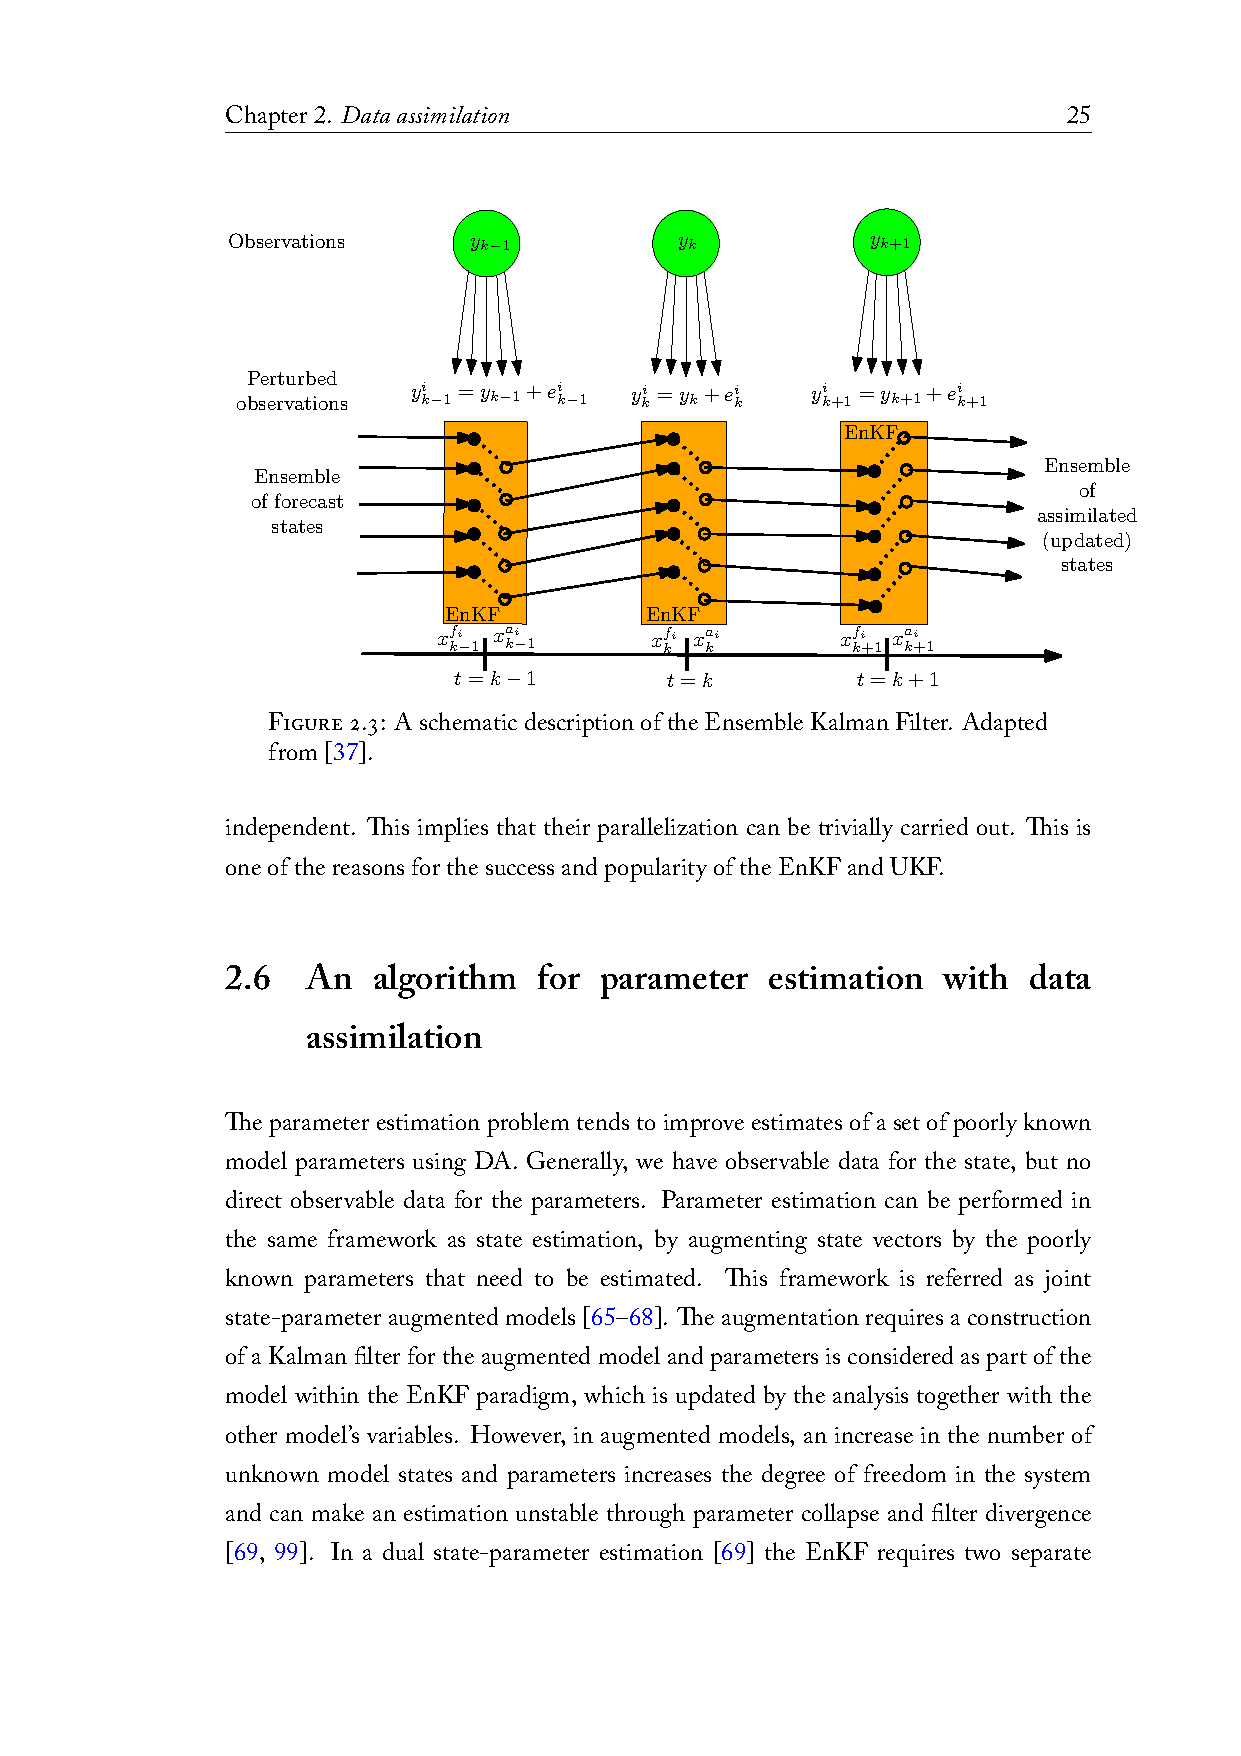
\includegraphics[width=\textwidth,trim = 3.5cm 22cm 3cm 3.5cm, clip]{kfchart.pdf}
%\caption{Fonctionnement schématique du EnKF. Issu de R. Lal.}
%\end{figure}
% 
%
%\paragraph
%\frametitle{Algorithme}
%Pour $k$ de 1 à $T/dt$ :
%
%
%\bigskip
%
%
%\begin{tabular}{p{3cm}|l}
%Analyse &$K_k = P^f_k\cdot H_k\cdot(H_k\cdot P^f_k\cdot H_k\trn + R_k)^{-1}$\\
%&$\x^a_k = \x^f_k + K_k\cdot(\y_k - H_k\cdot\x^f_k)$\\
%&$P^a_k = (I-K_k\cdot H_k)\cdot P^f_k$\\
%\end{tabular}
%
%
%\bigskip
%
%
%\begin{tabular}{p{3cm}|l}
%Prédiction &$\x^f_{k+1} = A_k\cdot \x^a_k$\\
%&$P^f_{k+1} = A_k\cdot P^a_k\cdot A_k\trn +Q_k$
%\end{tabular}
% 
%
%\paragraph
%\frametitle{Exemple : chute libre}
%$$\x_k=\left(\begin{matrix}x_k&x'_k&x''_k\end{matrix}\right)\trn$$
%
%$$A=\left(\begin{matrix}1&dt&dt^2\\0&1&dt\\0&0&1\end{matrix}\right)~~~~H=\left(\begin{matrix}1&0&0\\0&1&0\\0&0&1\end{matrix}\right)$$
%
%\begin{itemize}
%\item $g=-9.81 m.s^{-2}$,
%\item $dt=0.2 s$,
%\item $T=5 s$,
%\item $\x_1=\left(\begin{matrix}0&0&0\end{matrix}\right)\trn$,
%\item $w_k=1$, $w_k'=0.5$, $w_k''=0.25$ (écarts-types : perturbations),
%\item $v_k=5$, $v_k'=5$, $v_k''=10$ (écarts-types : erreurs de mesure).
%\end{itemize}
% 
%
%
%\paragraph
%\frametitle{Exemple : chute libre}
%\begin{figure}[!h]
%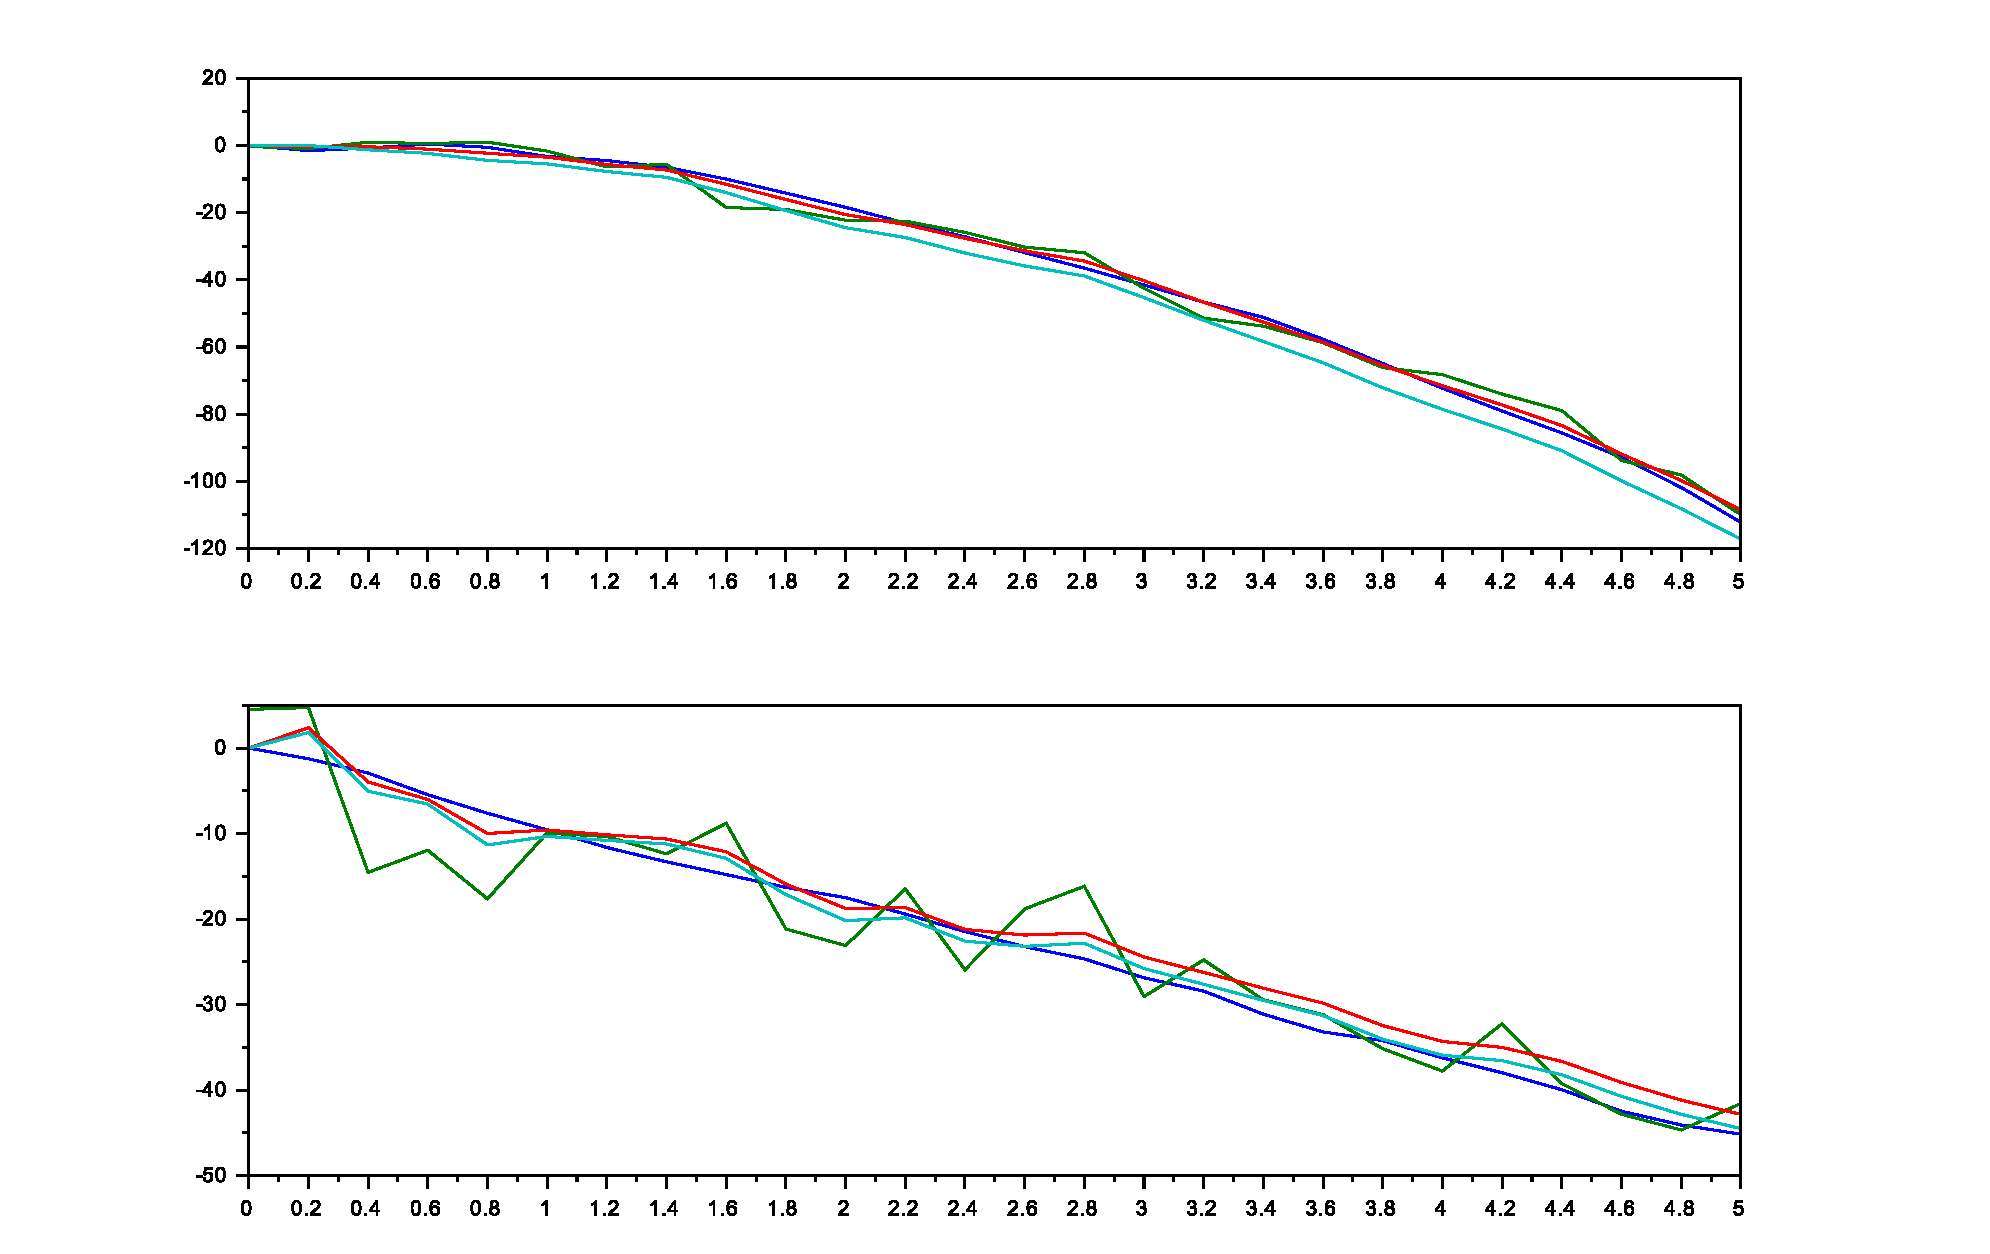
\includegraphics[width=\textwidth]{KalmanMobile.pdf}
%\caption{En bleu : $\x$ ;en vert : $\y$ ; en rouge : $\x^a$ ; en cyan : $\x^f$.}
%\end{figure}
% 
%
%
%\section{Ensemble Kalman Filter}
%
%\paragraph
%\frametitle{Filtre de Kalman à ensemble (EnKF)}
%Même principe que le KF, plus adapté aux processus non-linéaires.
%
%\eq{\left\{\begin{array}{l}\x_{k+1} = f(\x_k,\mathbf u_k)+\mathbf w_k\\\y_k=h(\x_k)+\mathbf v_k\end{array}\right.}
%
%
%Si la physique n'est pas connue, on considère que $\x$ est un processus aléatoire :
%
%\eq{x^f_{k+1}=x^f_k+\delta_k}
%
%où $\delta_k\sim\nor0{D_k}$.
%
% 
%
%\paragraph
%\frametitle{Filtre de Kalman à ensemble (EnKF)}
% À chaque pas :
%
%
%\bigskip
%
%
%\begin{itemize}
%\item<2-6>mesure $\y_k$
%\item<3-6>bruitage de la mesure $\y_k^i=\y_k+\mathbf e_k^i$, $i=1,...,q_{ens}$
%\item<4-6>analyse de l'état actuel $\x^{ai}_k=\x^{fi}_k+K_k(\y^i_k-h(\x^{fi}_k))$, $i=1,...,q_{ens}$
%\item<5-6>prédiction de l'état futur $\x^{fi}_{k+1}=f(\x^{ai}_k)$, $i=1,...,q_{ens}$
%\item<6>moyenne des prédictions $\overline{\x_k^f}$
%\end{itemize}
%\vspace{0.85cm}
% 
%
%\paragraph
%\frametitle{Filtre de Kalman à ensemble (EnKF)}
% À chaque pas :
%
%
%\bigskip
%
%
%\begin{itemize}
%\item mesure $\y_k$
%\item bruitage de la mesure $\y_k^i=\y_k+\mathbf e_k^i$, $i=1,...,q_{ens}$
%\item analyse de l'état actuel $\x^{ai}_k=\x^{fi}_k+K_k(\y^i_k-h(\x^{fi}_k))$, $i=1,...,q_{ens}$
%\item prédiction de l'état futur $\x^{fi}_{k+1}=f(\x^{ai}_k)$, $i=1,...,q_{ens}$
%\item moyenne des prédictions $\overline{\x_k^f}$
%\end{itemize}
%
%
%\bigskip
%
%
%\centering $\to$ algorithme parallélisable
% 
%
%\paragraph
%\frametitle{Filtre de Kalman à ensemble (EnKF)}
%\begin{figure}
%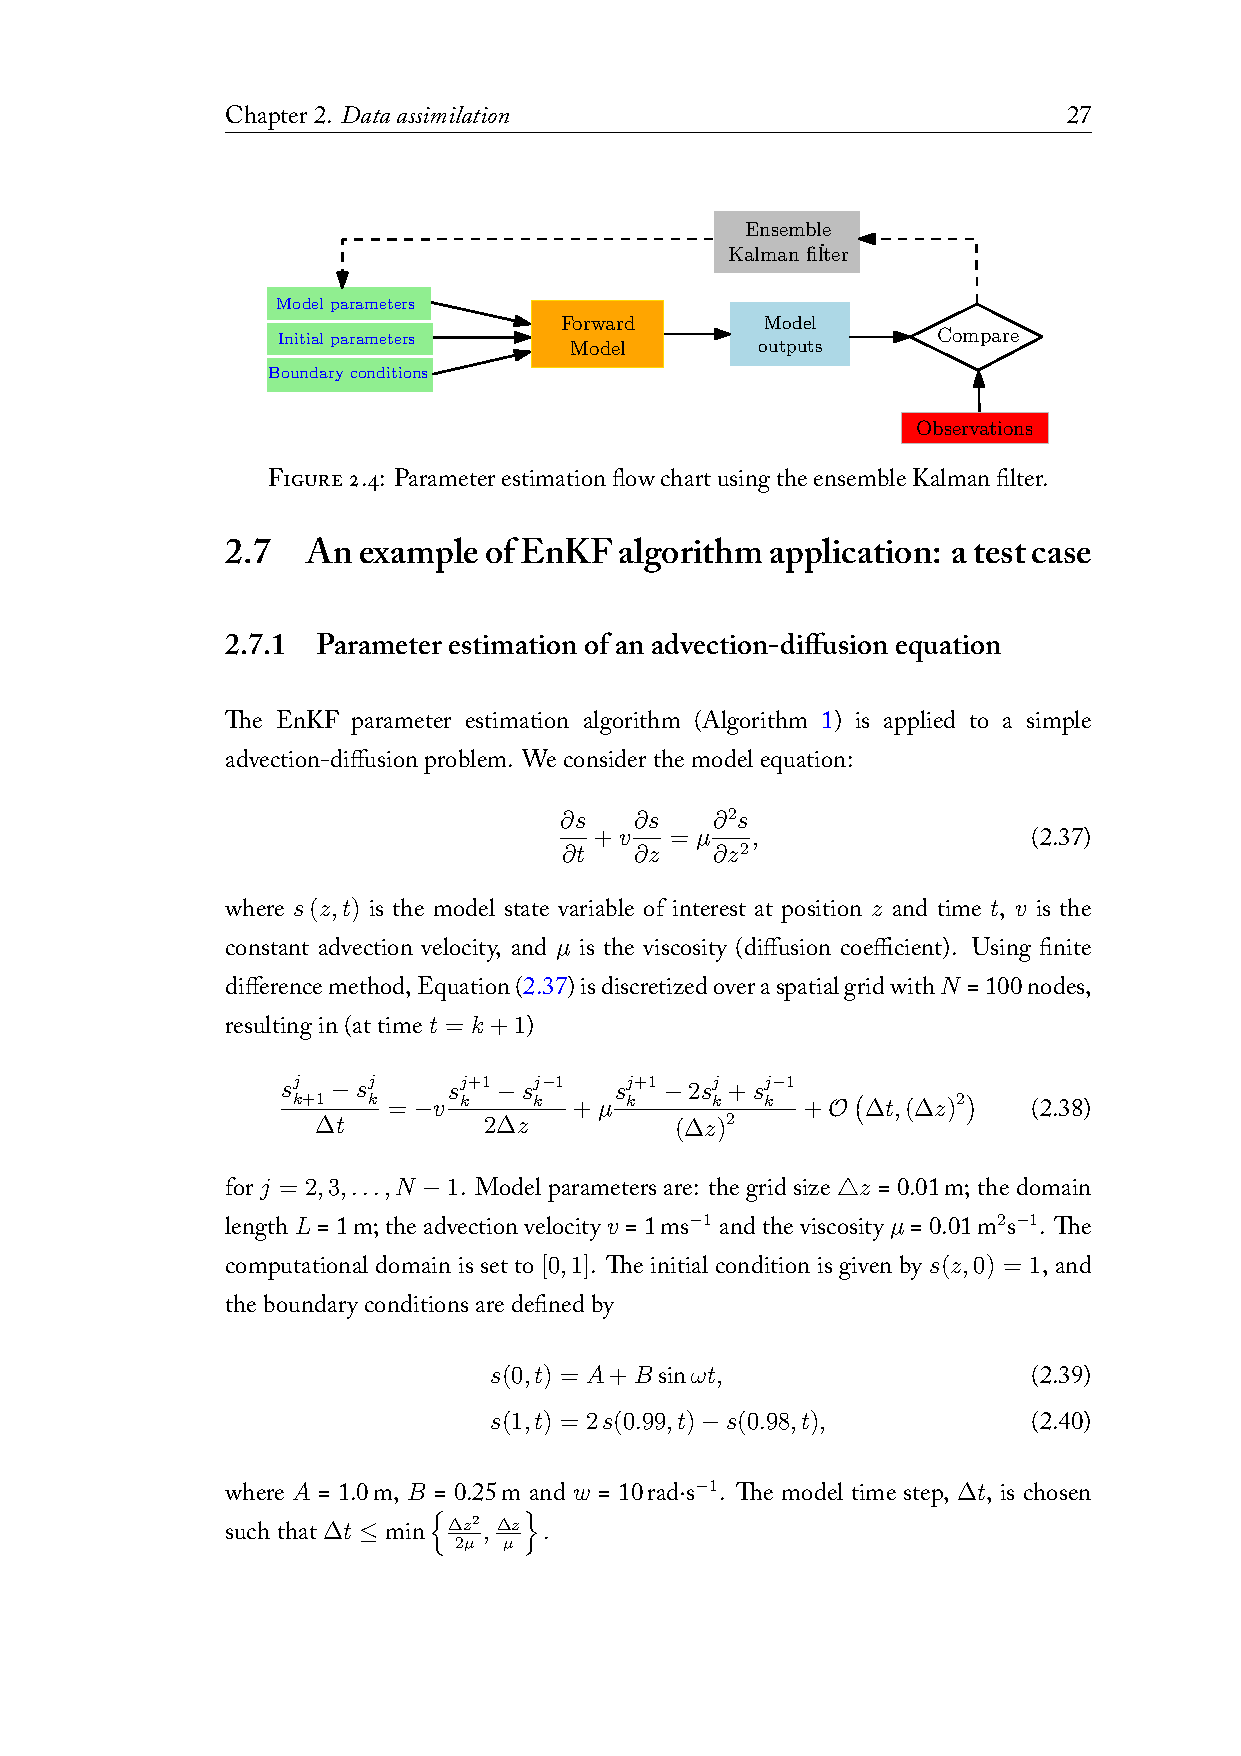
\includegraphics[width=\textwidth,trim = 3.85cm 18.1cm 1.8cm 3.5cm, clip]{enkfchart.pdf}
%\caption{Actualisation et prédiction du EnKF. Issu de R. Lal.}
%\end{figure}
% 
%
%\paragraph
%\frametitle{Exemple : chute libre}
%Dans les mêmes conditions que précédemment, on suppose qu'on ne connaît pas la physique, et on prend :
%$$\begin{array}{rl}D_k=&\left(\begin{matrix}(x_k-x_{k-1})^2&0&0\\0&(x'_k-x'_{k-1})^2&0\\0&0&dt\end{matrix}\right)\\=&\left(\begin{matrix}(x'_0dt+g(2k-1)dt^2)^2&0&0\\0&(gdt)^2&0\\0&0&dt\end{matrix}\right)\end{array}$$
% 
%
%\paragraph
%\frametitle{Exemple : chute libre}
%\begin{figure}[!h]
%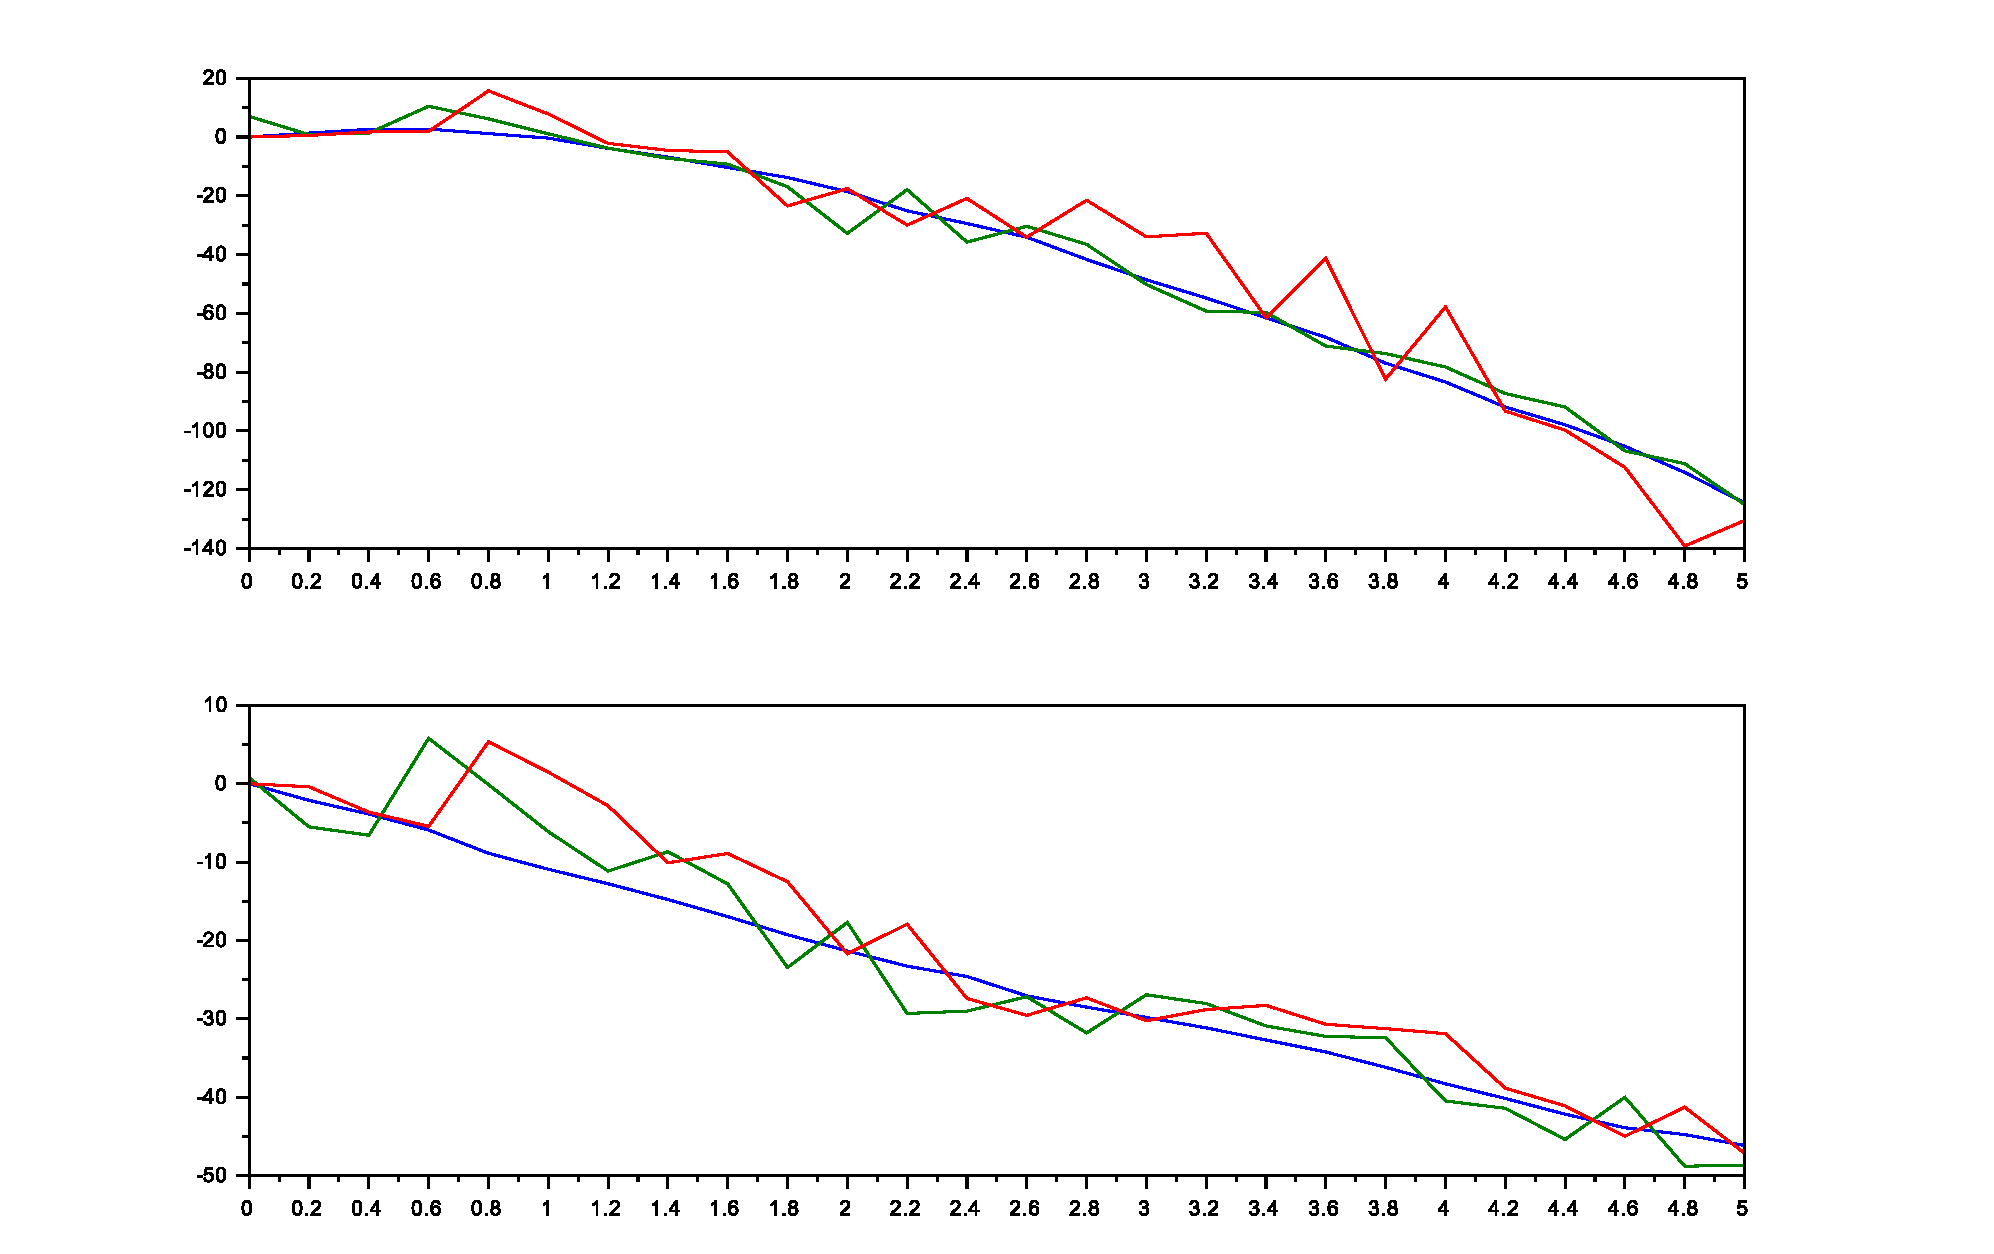
\includegraphics[width=\textwidth]{ENKalmanMobile.pdf}
%\caption{En bleu : $\x$ ; en vert : $\y$ ; en rouge : $\overline{\x^f}$.}
%\end{figure}
% 
%
%\paragraph
%\frametitle{Estimation de paramètres}
%Si le système est décrit par des paramètres non-mesurables $\mu$ et  par un état mesurable $\x=\x(\mu)$ , on peut vouloir estimer ces paramètres. Deux possibilités :
%
%
%\bigskip
%
%
%\begin{itemize}
%\item<2-3>algorithme EnKF sur $\x'=(\x, \mu)$ $\to$ instabilité
%\item<3>deux algorithmes EnKF en parallèle sur $\x$ et $\mu$
%\end{itemize}
%\vspace{1.4cm}
% 
%
%\paragraph
%\frametitle{Estimation de paramètres}
%Si le système est décrit par des paramètres non-mesurables $\mu$ et  par un état mesurable $\x=\x(\mu)$ , on peut vouloir estimer ces paramètres. Deux possibilités :
%
%
%\bigskip
%
%
%\begin{itemize}
%\item algorithme EnKF sur $\x'=(\x, \mu)$ $\to$ instabilité
%\item deux algorithmes EnKF en parallèle sur $\x$ et $\mu$
%\end{itemize}
%
%
%\bigskip
%
%
%Dans le second cas, on utilise à chaque pas l'estimation de $\mu$ pour celle de $\x$.
% 
%
%\section{}
%\paragraph
%\centering\textbf{\Large Merci pour votre attention !}
% 

\end{document} 